\documentclass[12pt,openright,oneside,a4paper,brazilian]{abntex2}

% --- Pacotes Básicos ---
\usepackage[T1]{fontenc}
\usepackage[utf8]{inputenc}
\usepackage{helvet} % Fonte Arial/Helvetica
\renewcommand{\familydefault}{\sfdefault} % Define a fonte sem serifa como padrão
\usepackage{graphicx}
\usepackage{microtype}
\usepackage{multirow}
\usepackage{rotating}
\usepackage{amsmath,amssymb}
\usepackage{siunitx}
\usepackage{float}
\usepackage{makeidx} % índice remissivo
\usepackage[table,xcdraw]{xcolor}
\makeindex


% --- Margens (ABNT: Superior/Esquerda 3cm, Inferior/Direita 2cm) ---
\usepackage[top=3cm, left=3cm, right=2cm, bottom=2cm]{geometry}

% --- Espaçamento de primeira linha (ABNT) ---
\setlength{\parindent}{1.5cm}

\newcommand{\norma}[1]{\textbf{#1}}

% --- Pacote e comando para destacar, ao longo do texto, os itens do ---
% --- roteiro (ROTEIRO_DE_ELABORAÇÃO_DO_PROJETO_ELÉTRICO...) que ainda ---
% --- não foram atendidos pelo grupo. Basta remover o \FALTA{...} ---
% --- quando o item correspondente for de fato elaborado. ---
\usepackage{xcolor}
\newcommand{\FALTA}[1]{%
  \par\noindent\fcolorbox{red}{yellow!15}{%
    \parbox{\dimexpr\linewidth-2\fboxsep-2\fboxrule}{%
      \small\textbf{[PENDENTE]:} #1}}\par\vspace{2mm}}

% --- Estilo de Cabeçalho e Rodapé (Logo superior direito, Página inferior direito) ---

\makepagestyle{estilo_personalizado}
% Cabeçalho ímpar/par: vazio no centro, vazio à esquerda, espaço de logo à direita

\makeoddhead{estilo_personalizado}{}{}{\IfFileExists{imagens/Logo_UEM.png}{
\includegraphics[width=2.2cm]{imagens/Logo_UEM.png}}{\textbf{UEM}}}


% Rodapé ímpar/par: vazio no centro, vazio à esquerda, número da página à direita
\makeoddfoot{estilo_personalizado}{}{}{\thepage}
\makeevenfoot{estilo_personalizado}{}{}{\thepage}

% --- Títulos e Subtítulos em Negrito ---
\renewcommand{\ABNTEXchapterfont}{\sffamily\bfseries}
\renewcommand{\ABNTEXchapterfontsize}{\large}
\renewcommand{\ABNTEXsectionfont}{\sffamily\bfseries}
\renewcommand{\ABNTEXsectionfontsize}{\large}

\renewcommand{\chaptername}{Módulo}
\setlength{\afterchapskip}{\baselineskip} 

\makeatletter
\addto\captionsbrazilian{
  \renewcommand{\chaptermark}[1]{%
    \markright{%
      \ifnum \c@secnumdepth >\m@ne
        \if@mainmatter
          \thechapter\ --\ %  <-- Altera o texto aqui
        \fi
      \fi
      #1}}%
}

% --- Citações (ABNT) ---
\usepackage[alf]{abntex2cite}

% --- Arquivo de Referências (Embutido para facilidade) ---
% Referências em referencias.bib (revisado). Os itens marcados com "CONFERIR"
% no .bib devem ser checados contra o documento original (capa da NTC,
% ficha catalográfica, catálogo da ABNT).


\hypersetup{
    colorlinks=true,       % Transforma as caixas em textos coloridos
    linkcolor=black,       % Cor dos links internos (tabelas, figuras)
    citecolor=black,       % Cor das citações (pode trocar para blue se preferir)
    urlcolor=black         % Cor dos links de internet
}

% --- Informações de Capa e Folha de Rosto (Contra Capa) ---
\titulo{Motor CC shunt de 1,5 HP com controle de velocidade e torque}
\autor{Antonio Nicolas Irmani\\
        João Marcos Conti Checom\\
        Juan Antonio Marques Fogaça de Oliveira\\
        Henry Barbosa Azevedo}
\local{\textbf{Maringá -- Paraná}}
\data{2026}
\orientador{Glaucio Pedro de Alcantara}
\instituicao{%
  \textbf{Universidade Estadual de Maringá - UEM}
  \par
  Departamento de Engenharia Química 
  \par
  Engenharia Elétrica}
\tipotrabalho{Trabalho acadêmico}
\preambulo{Trabalho acadêmico apresentado à Universidade Estadual de Maringá, no curso de Engenharia Elétrica.}

\begin{document}

% Retira espaço extra obsoleto entre as frases.
\frenchspacing

% ----------------------------------------------------------
% ELEMENTOS PRÉ-TEXTUAIS
% ----------------------------------------------------------

% ----------------------------------------------------------
% CAPA CUSTOMIZADA
% ----------------------------------------------------------
\begin{capa}
    \begin{center}
        
        % --- Cabeçalho: Logo e Instituição ---
        % O minipage divide a parte superior em duas colunas. 
        \begin{minipage}[c]{0.2\textwidth}
            \centering
            % Quando tiver a logo, apague o comando \rule abaixo e descomente o \includegraphics
            \IfFileExists{imagens/Logo.png}{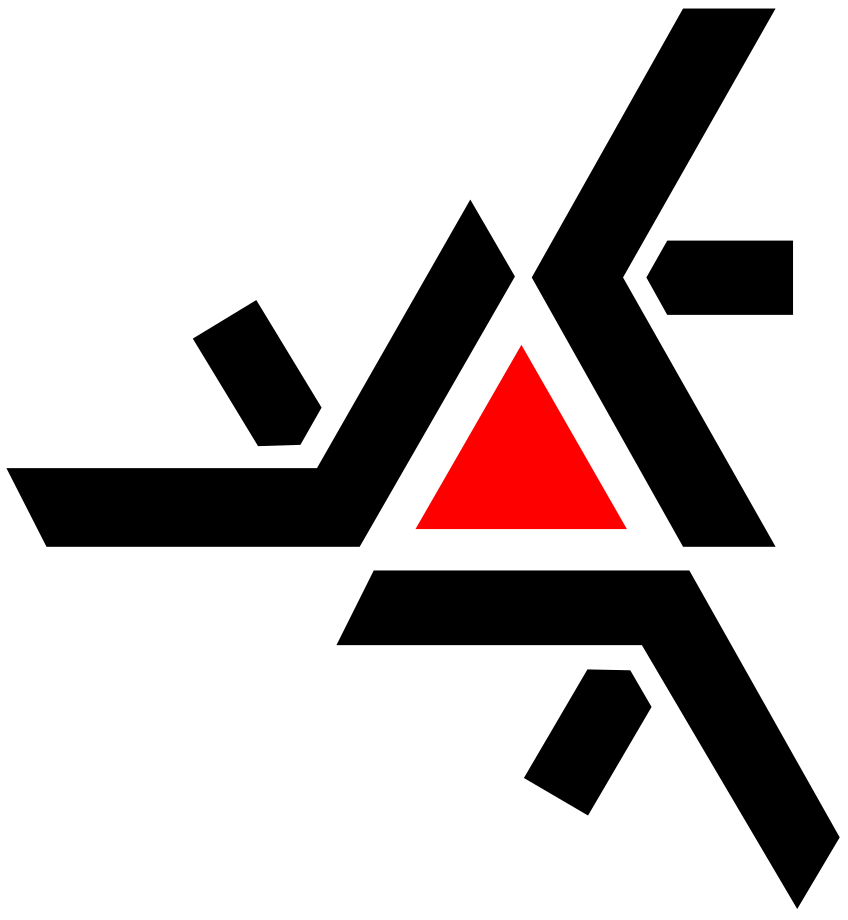
\includegraphics[width=2.8cm]{imagens/Logo.png}}{\textbf{UEM}} % Logo Capa
            %\rule{2.5cm}{3.2cm} % Retângulo preto simulando a imagem da logo
        \end{minipage}%
        \begin{minipage}[c]{0.75\textwidth}
            \centering
            \textbf{UNIVERSIDADE ESTADUAL DE MARINGÁ - UEM}\\
            \textbf{DEPARTAMENTO DE ENGENHARIA QUÍMICA}\\
            \textbf{ENGENHARIA ELÉTRICA}\\
            \textbf{MÁQUINAS ELÉTRICAS I}
        \end{minipage}
        
        \vspace*{3.5cm} % Espaçamento vertical até os autores
        
        % --- Lista de Autores ---
        Antonio Nicolas Irmani\\
        João Marcos Conti Checom\\
        Juan Antonio Marques Fogaça de Oliveira\\
        Henry Barbosa Azevedo
        
        \vspace*{4.5cm} % Espaçamento vertical até o título
        
        % --- Título do Trabalho ---
        \textbf{\large{Motor CC shunt de 1,5 HP com controle de velocidade e torque}}
        
        \vfill % Este comando empurra automaticamente o bloco abaixo para o limite inferior da página
        
        % --- Local e Data ---
        \textbf{MARINGÁ -- PR}\\
        \textbf{2026}
        
    \end{center}
\end{capa}


\imprimirfolhaderosto

% Elementos pré-textuais: ordem e espaçamentos do original.
% O bookmark manual foi omitido para evitar o erro do MiKTeX.
\tableofcontents*
\cleardoublepage

\frontmatter
\pretextual
\pagenumbering{arabic}

\begin{agradecimentos}
\addcontentsline{toc}{section}{I.\hspace{1.82cm}Agradecimentos}
\hspace{1.27cm} [INSERIR AGRADECIMENTOS.]
\end{agradecimentos}
\cleardoublepage

\addcontentsline{toc}{section}{II.\hspace{1.71cm}Lista de Ilustrações}
\listoffigures*
\cleardoublepage

\addcontentsline{toc}{section}{III.\hspace{1.61cm}Lista de Tabelas}
\listoftables*
\cleardoublepage

\addcontentsline{toc}{section}{IV.\hspace{1.61cm}Glossário}
\chapter*{Glossário}
\begin{description}[itemsep=0.01em]
    \item[\textbf{UEM}] Universidade Estadual de Maringá.
\end{description}
\cleardoublepage

\addcontentsline{toc}{section}{V.\hspace{1.74cm}Índice}
\printindex
\cleardoublepage

\textual
\pagestyle{estilo_personalizado}
\aliaspagestyle{chapter}{estilo_personalizado}
\mainmatter
\pagenumbering{arabic}

\chapter{INTRODUÇÃO}
\section{Contextualização das máquinas de corrente contínua}
\FALTA{Desenvolver esta seção com fundamentação, cálculos, diagramas e/ou evidências aplicáveis.}
\section{Objetivo geral e objetivos específicos}
\FALTA{Desenvolver esta seção com fundamentação, cálculos, diagramas e/ou evidências aplicáveis.}
\section{Justificativa do projeto}
\FALTA{Desenvolver esta seção com fundamentação, cálculos, diagramas e/ou evidências aplicáveis.}

\chapter{DESCRIÇÃO DO PROBLEMA E REQUISITOS}
\section{Descrição do desafio proposto}
\FALTA{Desenvolver esta seção com fundamentação, cálculos, diagramas e/ou evidências aplicáveis.}
\section{Requisitos construtivos do motor}
\FALTA{Desenvolver esta seção com fundamentação, cálculos, diagramas e/ou evidências aplicáveis.}
\section{Requisitos de partida e funcionamento}
\FALTA{Desenvolver esta seção com fundamentação, cálculos, diagramas e/ou evidências aplicáveis.}
\section{Requisitos de controle de velocidade, medição de RPM e reversão}
\FALTA{Desenvolver esta seção com fundamentação, cálculos, diagramas e/ou evidências aplicáveis.}

\chapter{FUNDAMENTAÇÃO TEÓRICA}
\section{Princípio de funcionamento do motor CC shunt}
\FALTA{Desenvolver esta seção com fundamentação, cálculos, diagramas e/ou evidências aplicáveis.}
\section{Estrutura e componentes do motor CC shunt}
\FALTA{Desenvolver esta seção com fundamentação, cálculos, diagramas e/ou evidências aplicáveis.}
\section{Excitação em derivação (shunt) e circuito de campo}
\FALTA{Desenvolver esta seção com fundamentação, cálculos, diagramas e/ou evidências aplicáveis.}
\section{Força contraeletromotriz e conjugado eletromagnético}
\FALTA{Desenvolver esta seção com fundamentação, cálculos, diagramas e/ou evidências aplicáveis.}
\section{Equações de regime permanente do motor shunt}
\FALTA{Desenvolver esta seção com fundamentação, cálculos, diagramas e/ou evidências aplicáveis.}
\section{Comutação, escovas e comutador}
\FALTA{Desenvolver esta seção com fundamentação, cálculos, diagramas e/ou evidências aplicáveis.}
\section{Enrolamento imbricado da armadura}
\FALTA{Desenvolver esta seção com fundamentação, cálculos, diagramas e/ou evidências aplicáveis.}
\section{Enrolamento imbricado simplex e caminhos paralelos}
\FALTA{Desenvolver esta seção com fundamentação, cálculos, diagramas e/ou evidências aplicáveis.}
\section{Enrolamento imbricado progressivo}
\FALTA{Desenvolver esta seção com fundamentação, cálculos, diagramas e/ou evidências aplicáveis.}

\chapter{CARACTERÍSTICAS E DIMENSIONAMENTO DO MOTOR}
\section{Definição da configuração construtiva shunt}
\FALTA{Desenvolver esta seção com fundamentação, cálculos, diagramas e/ou evidências aplicáveis.}
\section{Sistema magnético de dois polos}
\FALTA{Desenvolver esta seção com fundamentação, cálculos, diagramas e/ou evidências aplicáveis.}
\section{Rotor com oito ranhuras}
\FALTA{Desenvolver esta seção com fundamentação, cálculos, diagramas e/ou evidências aplicáveis.}
\section{Comutador com oito segmentos}
\FALTA{Desenvolver esta seção com fundamentação, cálculos, diagramas e/ou evidências aplicáveis.}
\section{Distribuição das bobinas e conexões do enrolamento}
\FALTA{Desenvolver esta seção com fundamentação, cálculos, diagramas e/ou evidências aplicáveis.}
\section{Parâmetros elétricos e mecânicos do motor shunt}
\FALTA{Desenvolver esta seção com fundamentação, cálculos, diagramas e/ou evidências aplicáveis.}
\section{Estimativas de corrente, conjugado e velocidade no motor shunt}
\FALTA{Desenvolver esta seção com fundamentação, cálculos, diagramas e/ou evidências aplicáveis.}

\chapter{ALTERNATIVAS E SOLUÇÕES SELECIONADAS}
\section{Dimensionamento e alimentação do campo shunt}
\FALTA{Desenvolver esta seção com fundamentação, cálculos, diagramas e/ou evidências aplicáveis.}
\section{Soluções de controle de velocidade para o motor shunt}
\FALTA{Desenvolver esta seção com fundamentação, cálculos, diagramas e/ou evidências aplicáveis.}
\section{Seleção do sistema de medição de rotação}
\FALTA{Desenvolver esta seção com fundamentação, cálculos, diagramas e/ou evidências aplicáveis.}
\section{Seleção do sistema de reversão de rotação}
\FALTA{Desenvolver esta seção com fundamentação, cálculos, diagramas e/ou evidências aplicáveis.}
\section{Justificativa da arquitetura escolhida}
\FALTA{Desenvolver esta seção com fundamentação, cálculos, diagramas e/ou evidências aplicáveis.}

\chapter{SISTEMAS ELETRÔNICOS AUXILIARES}
\section{Controle PWM utilizando o temporizador 555}
\FALTA{Desenvolver esta seção com fundamentação, cálculos, diagramas e/ou evidências aplicáveis.}
\section{Estágio de acionamento do motor}
\FALTA{Desenvolver esta seção com fundamentação, cálculos, diagramas e/ou evidências aplicáveis.}
\section{Tacômetro digital com microcontrolador}
\FALTA{Desenvolver esta seção com fundamentação, cálculos, diagramas e/ou evidências aplicáveis.}
\section{Exibição de velocidade em display LCD}
\FALTA{Desenvolver esta seção com fundamentação, cálculos, diagramas e/ou evidências aplicáveis.}
\section{Sistema de reversão de rotação}
\FALTA{Desenvolver esta seção com fundamentação, cálculos, diagramas e/ou evidências aplicáveis.}
\section{Integração dos circuitos e alimentação shunt}
\FALTA{Desenvolver esta seção com fundamentação, cálculos, diagramas e/ou evidências aplicáveis.}

\chapter{METODOLOGIA DE DESENVOLVIMENTO}
\section{Planejamento e modelagem teórica}
\FALTA{Desenvolver esta seção com fundamentação, cálculos, diagramas e/ou evidências aplicáveis.}
\section{Seleção de materiais e componentes}
\FALTA{Desenvolver esta seção com fundamentação, cálculos, diagramas e/ou evidências aplicáveis.}
\section{Construção do estator e do rotor}
\FALTA{Desenvolver esta seção com fundamentação, cálculos, diagramas e/ou evidências aplicáveis.}
\section{Implementação do enrolamento imbricado progressivo}
\FALTA{Desenvolver esta seção com fundamentação, cálculos, diagramas e/ou evidências aplicáveis.}
\section{Montagem do comutador e das escovas}
\FALTA{Desenvolver esta seção com fundamentação, cálculos, diagramas e/ou evidências aplicáveis.}
\section{Implementação dos circuitos eletrônicos}
\FALTA{Desenvolver esta seção com fundamentação, cálculos, diagramas e/ou evidências aplicáveis.}
\section{Integração e verificação do protótipo}
\FALTA{Desenvolver esta seção com fundamentação, cálculos, diagramas e/ou evidências aplicáveis.}

\chapter{ENSAIOS E RESULTADOS EXPERIMENTAIS}
\section{Verificação da partida autônoma}
\FALTA{Desenvolver esta seção com fundamentação, cálculos, diagramas e/ou evidências aplicáveis.}
\section{Medição da velocidade de rotação}
\FALTA{Desenvolver esta seção com fundamentação, cálculos, diagramas e/ou evidências aplicáveis.}
\section{Verificação do controle PWM no osciloscópio}
\FALTA{Desenvolver esta seção com fundamentação, cálculos, diagramas e/ou evidências aplicáveis.}
\section{Relação entre ciclo de trabalho e RPM}
\FALTA{Desenvolver esta seção com fundamentação, cálculos, diagramas e/ou evidências aplicáveis.}
\section{Teste de reversão do sentido de rotação}
\FALTA{Desenvolver esta seção com fundamentação, cálculos, diagramas e/ou evidências aplicáveis.}
\section{Análise dos resultados e limitações}
\FALTA{Desenvolver esta seção com fundamentação, cálculos, diagramas e/ou evidências aplicáveis.}

\chapter{CONCLUSÕES E CONSIDERAÇÕES FINAIS}
\FALTA{Redigir as conclusões com base nos resultados reais do protótipo.}

\postextual
\chapter*{REFERÊNCIAS}
\addcontentsline{toc}{chapter}{REFERÊNCIAS}
\FALTA{Inserir referências bibliográficas efetivamente consultadas.}
\appendix
\chapter{Diagramas elétricos}
\FALTA{Inserir os diagramas definitivos.}
\chapter{Código do microcontrolador}
\FALTA{Inserir o código utilizado no tacômetro.}
\chapter{Registros fotográficos e medições}
\FALTA{Inserir registros obtidos durante a montagem e os ensaios.}
\end{document}